%--------------------------------------
% Create title frame
\titleframe
%--------------------------------------
% Table of contents
\begin{frame}{Sommaire}
\begin{tikzpicture}[remember picture, overlay]
\node[opacity=.4, inner sep=0pt]
    at(current page.center){
\includegraphics[width=16cm]{resources/background.jpg}};
\end{tikzpicture}

  \setbeamertemplate{section in toc}[sections numbered]
  \tableofcontents[hideallsubsections]
\end{frame}

%==============================================
\section*{Introduction}
%==============================================

\begin{frame}[fragile=singleslide]{\insertsectionhead}
\begin{tikzpicture}[remember picture, overlay]
\node[opacity=.4, inner sep=0pt]
    at(current page.center){
\includegraphics[width=16cm]{resources/background.jpg}};
\node[opacity=1, inner sep=0pt]
    at(325pt, -120pt){
\includegraphics[width=5.5cm]{resources/light.png}};
\node[opacity=1, inner sep=0pt]
    at(275pt, 10pt){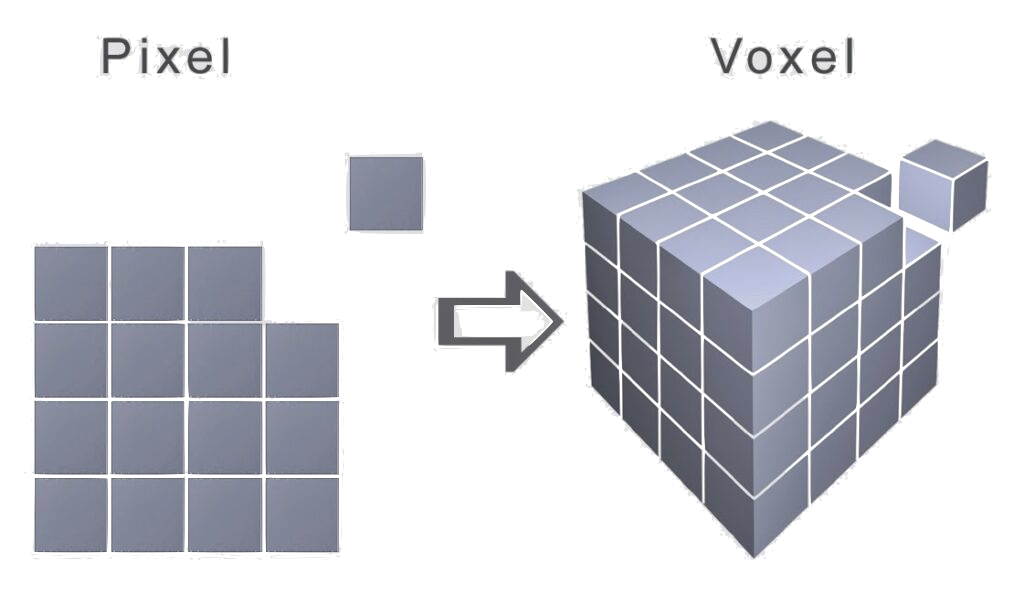
\includegraphics[width=8cm]{resources/voxel.png}};
\end{tikzpicture}

    \vspace{.5cm}
    \textbf{Les utilisations:}
    \vspace{.2cm}
    \begin{itemize}
      \item Modélisation
      \vspace{.2cm}
      \item Simulation physique
        \begin{itemize}
          \vspace{.1cm}
          \item De nouvelles simulations rendues possibles
          \vspace{.05cm}
        \end{itemize}
      \item Eclairage volumétrique
    \end{itemize}

\end{frame}

%==============================================
\section{État de l'art}
%==============================================

\begin{frame}[fragile=singleslide]{\insertsectionhead}
\begin{tikzpicture}[remember picture, overlay]
\node[opacity=.4, inner sep=0pt]
    at(current page.center){
\includegraphics[width=16cm]{resources/background.jpg}};
\node[opacity=1, inner sep=0pt]
    at(130pt,-20pt){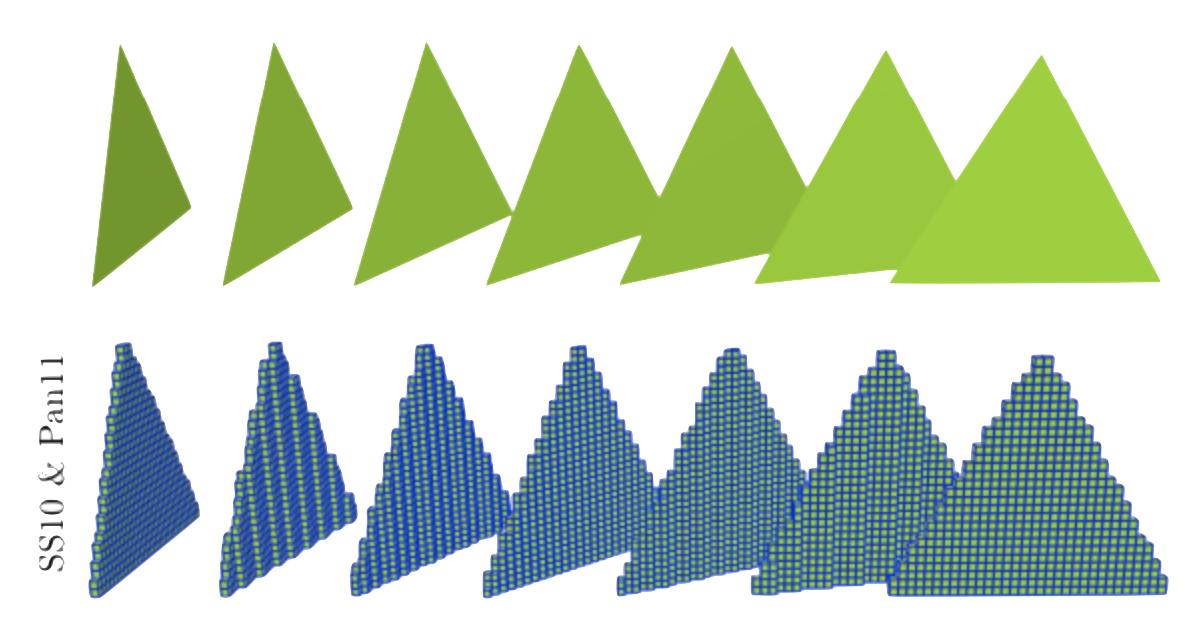
\includegraphics[width=10.5cm]{resources/triangles.png}};
\node[opacity=1, inner sep=0pt]
    at(370pt,-25pt){
\includegraphics[width=3.5cm]{resources/tunneling.png}};
\end{tikzpicture}

\end{frame}

%==============================================
\section{Etude de l'article}
%==============================================

\subsection{Spécificité de l'algorithme}

\begin{frame}[fragile=singleslide]{\insertsectionhead}
\begin{tikzpicture}[remember picture, overlay]
\node[opacity=.4, inner sep=0pt]
    at(current page.center){
\includegraphics[width=16cm]{resources/background.jpg}};
\end{tikzpicture}

  \framesubtitle{\insertsubsectionhead}
  \begin{columns}[T,onlytextwidth]
    \column{0.1\textwidth}
    \begin{figure}
      \begin{subfigure}{5.5\textwidth}
        \frame{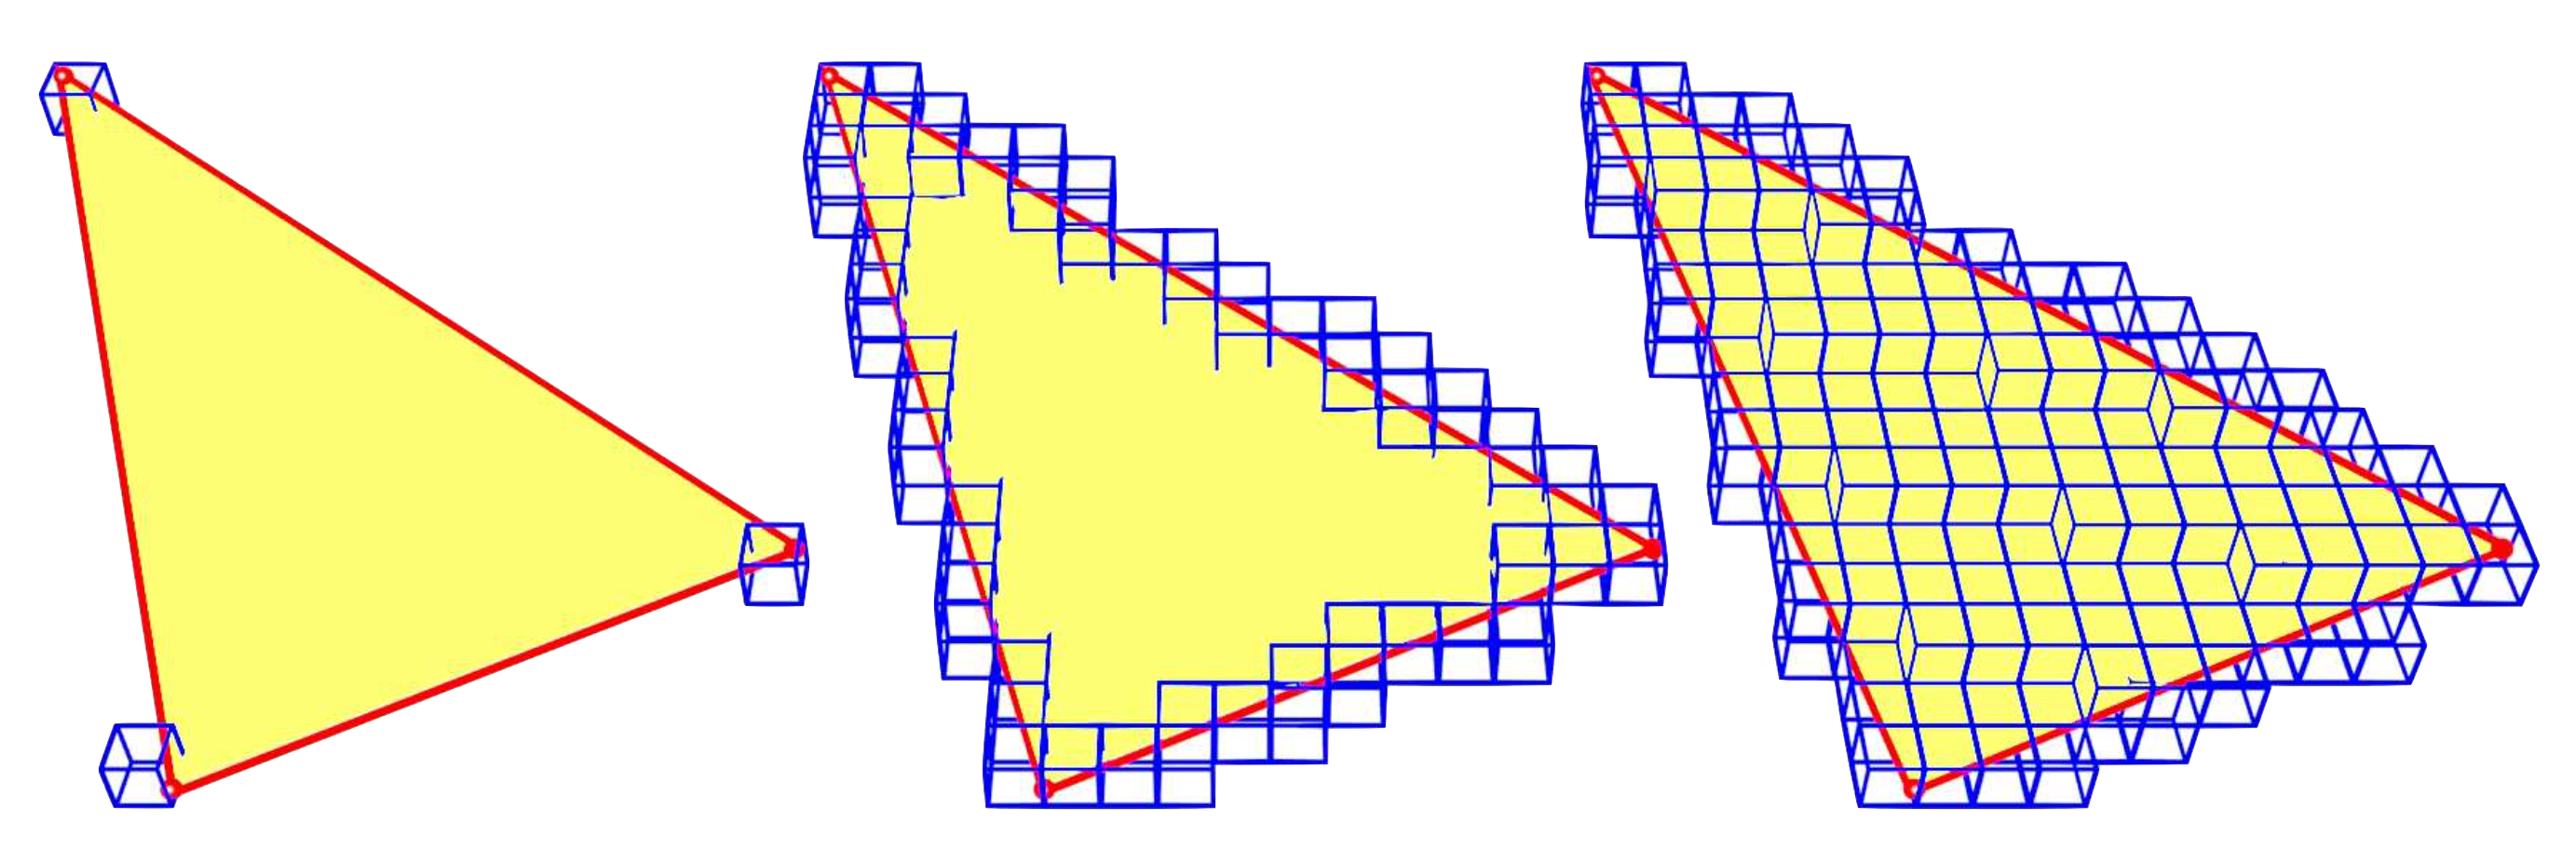
\includegraphics[width=\textwidth]{resources/voxelization_steps.png}}
        \caption*{Etapes de la voxelization}
      \end{subfigure}
    \end{figure}
    \column{0.4\textwidth}
    \begin{block}{MarkLineILV}
        Voxelization des côtés
    \end{block}
    \begin{block}{FillInterior}
        Voxelization de l'intérieur
    \end{block}
  \end{columns}
\end{frame}

%--------------------------------------
\subsection{3D voxelization ? scanlines ?}

\begin{frame}[fragile=singleslide]{\insertsectionhead}
\begin{tikzpicture}[remember picture, overlay]
\node[opacity=.4, inner sep=0pt]
    at(current page.center){
\includegraphics[width=17cm]{resources/background.jpg}};
\end{tikzpicture}

  \framesubtitle{\insertsubsectionhead}
  \begin{center}
      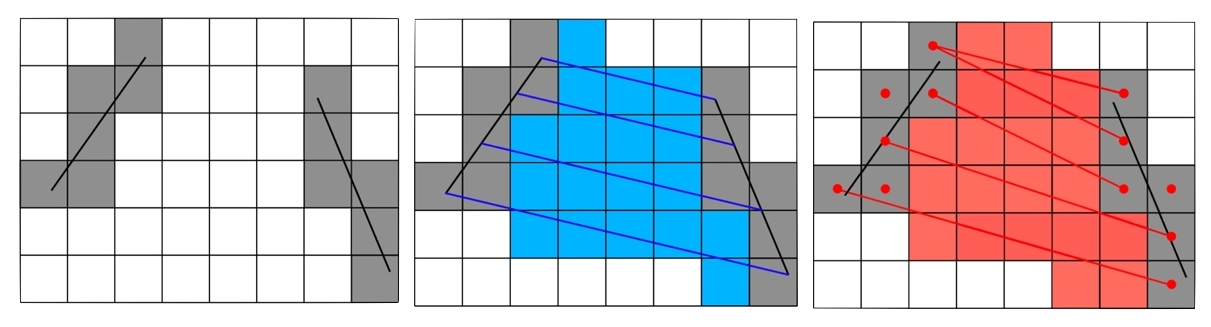
\includegraphics[scale=0.34]{resources/scanlines.png}
  \end{center}
  \vspace{1cm}
\end{frame}

%--------------------------------------
\subsection{Points clés}

\begin{frame}[fragile=singleslide]{\insertsectionhead}
\begin{tikzpicture}[remember picture, overlay]
\node[opacity=.4, inner sep=0pt]
    at(current page.center){
\includegraphics[width=16cm]{resources/background.jpg}};
\end{tikzpicture}

  \framesubtitle{\insertsubsectionhead}
  \begin{itemize}
      \item Optimisation en temps
      \item Parfaitement compatible avec le multithreading
      \item Plus on a de triangles plus c'est relativement rapide
      \item la discrétisation des entiers permet l’optimisation des temps de calcul
    \end{itemize}
    \vspace{0.6cm}
    \begin{center}
        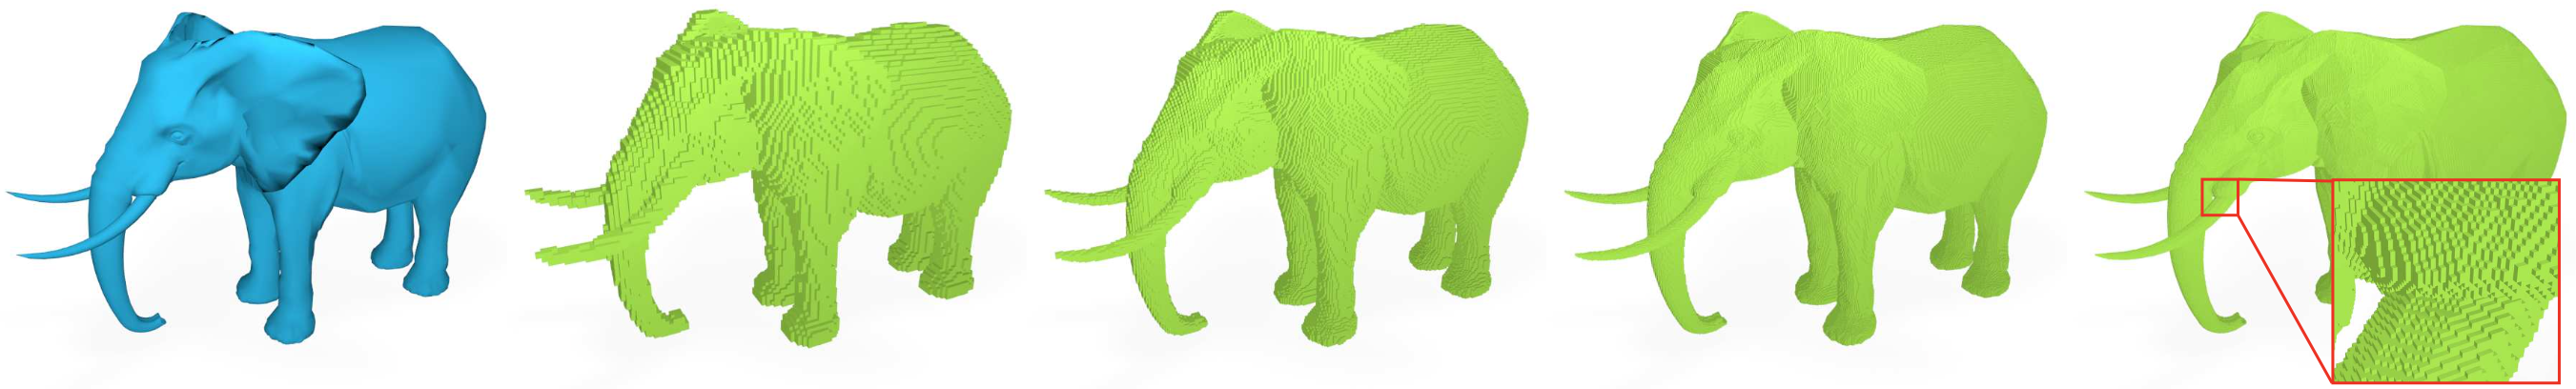
\includegraphics[scale=0.15]{resources/elephant.png}
    \end{center}
\end{frame}

%==============================================
\section{Prototypage}
%==============================================

\subsection{Plan initial}

\begin{frame}[fragile=singleslide]{\insertsectionhead}
\begin{tikzpicture}[remember picture, overlay]
\node[opacity=.4, inner sep=0pt]
    at(current page.center){
\includegraphics[width=16cm]{resources/background.jpg}};
\end{tikzpicture}

  \framesubtitle{\insertsubsectionhead}
  \begin{columns}[T,onlytextwidth]
    \column{0.4\textwidth}
    \vspace{0.6cm}
      \begin{itemize}
        \item Voxelization d'un triangle
        \vspace{.3cm}
        \item Utiliser OpenGL
        \vspace{.3cm}
        \item Prototypage 2D
      \end{itemize}
    \column{0.4\textwidth}
      
\includegraphics[scale=0.5]{resources/opengl_logo.png}
  \end{columns}
  \vfill
  \vfill
  \hspace{0.2cm}
  {\large Tout semblait simple et clair}
\end{frame}

%--------------------------------------
\subsection{Premiers résultats}

\begin{frame}[fragile=singleslide]{\insertsectionhead}
\begin{tikzpicture}[remember picture, overlay]
\node[opacity=.4, inner sep=0pt]
    at(current page.center){
\includegraphics[width=16cm]{resources/background.jpg}};
\end{tikzpicture}

  \framesubtitle{\insertsubsectionhead}
  \begin{itemize}
    \item Reprise en main d'openGL
    \vspace{.3cm}
    \item Rendu du triangle à l'écran très satisfaisante
    \vspace{.3cm}
    \item Voxelization des côtés se fait rapidement
  \end{itemize}
  \vspace{.4cm}
  \begin{figure}
        \begin{subfigure}{0.6\textwidth}
          \frame{
\includegraphics[width=\textwidth]{resources/voxelization_edge.png}}
          \caption*{Voxelization des côtés}
        \end{subfigure}
      \end{figure}
\end{frame}

%--------------------------------------
\subsection{Difficultés rencontrées}

\begin{frame}[fragile=singleslide]{\insertsectionhead}
\begin{tikzpicture}[remember picture, overlay]
\node[opacity=.4, inner sep=0pt]
    at(current page.center){
\includegraphics[width=16cm]{resources/background.jpg}};
\end{tikzpicture}

  \framesubtitle{\insertsubsectionhead}
  \begin{columns}[T,onlytextwidth]
    \column{0.4\textwidth}
      \vspace{.6cm}
      \begin{itemize}
        \item Apparition du problème de la pyramide
        \vspace{.3cm}
        \item La méthode naïve marche étonnamment mieux avec une couverture parfaite
      \end{itemize}
    \column{0.6\textwidth}
    \begin{figure}
        \begin{subfigure}{.8\textwidth}
          \frame{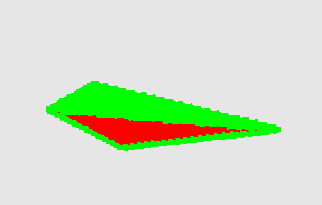
\includegraphics[width=\textwidth]{resources/pyramide_curse.png}}
          \caption*{Problème de la pyramide}
        \end{subfigure}
      \end{figure}
  \end{columns}
\end{frame}

%--------------------------------------
\subsection{Éclaircissement sur les zones d'ombres}

\begin{frame}[fragile=singleslide]{\insertsectionhead}
\begin{tikzpicture}[remember picture, overlay]
\node[opacity=.4, inner sep=0pt]
    at(current page.center){
\includegraphics[width=16cm]{resources/background.jpg}};
\end{tikzpicture}

  \framesubtitle{\insertsubsectionhead}
  \begin{columns}[T,onlytextwidth]
    \column{0.5\textwidth}
      \begin{itemize}
        \vspace{.55cm}
        \item Manque de détail dans les cas 2D
        \vspace{.3cm}
        \item Choix d’utilisation de Bresenham dans les cas 2D
        \vspace{.3cm}
        \item Des parties de l'algorithme ne sont pas détaillées(mettre image avec encadrés rouges
      \end{itemize}
    \column{0.6\textwidth}
    \begin{figure}
        \begin{subfigure}{.9\textwidth}
          \frame{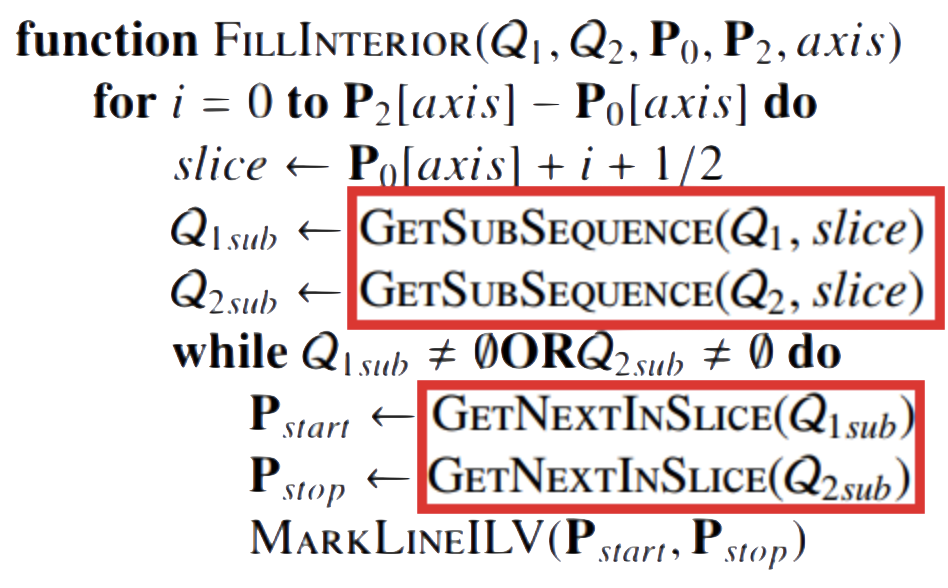
\includegraphics[width=.9\textwidth]{resources/subSequence.png}}
        \end{subfigure}
      \end{figure}
  \end{columns}
\end{frame}

%==============================================
\section{Résultats \& Benchmark}
%==============================================

\subsection{Quelques chiffres en comparaison}

\begin{frame}[fragile=singleslide]{\insertsectionhead}
\begin{tikzpicture}[remember picture, overlay]
\node[opacity=.4, inner sep=0pt]
    at(current page.center){
\includegraphics[width=16cm]{resources/background.jpg}};
\end{tikzpicture}

  \framesubtitle{\insertsubsectionhead}
  \begin{table}
    \centering
    \begin{tabular}{@{} lcccc @{}}
      \toprule
      & 100 & 1000  & 10000 & couverture
      & & triangles & triangles  & triangles & en \% \\
      \midrule
      Scanline Optimales  & 2.316 & 20.114 & 209.718 & 92.11 \\
      Scanline Naïves  & 4.35 & 45.584 & 444.665 & 100 \\
      \bottomrule
    \end{tabular}
  \end{table}
  \vspace{0.6cm}
  {\raggedleft\vfill\itshape\Longstack[l]{%
  \textbf{Et ensuite place à la démo !}
}\par}
\end{frame}

%--------------------------------------
\subsection{Perspectives d'évolution}

\begin{frame}[fragile=singleslide]{\insertsectionhead}
\begin{tikzpicture}[remember picture, overlay]
\node[opacity=.4, inner sep=0pt]
    at(current page.center){
\includegraphics[width=16cm]{resources/background.jpg}};
\node[opacity=.9, inner sep=0pt, rotate=-40]
at (280pt,-30pt){
\includegraphics[width=8cm]{resources/lit.png}};
\end{tikzpicture}


  \framesubtitle{\insertsubsectionhead}
  \begin{itemize}
    \item Utiliser CUDA
  \end{itemize}
  \hfill
  \begin{itemize}
    \item Changer de langage
  \end{itemize}
  \hfill
  \begin{itemize}
    \item Passer sur du multithread
  \end{itemize}
\end{frame}

%--------------------------------------
\subsection{Conclusion}

\begin{frame}[fragile=singleslide]{\insertsectionhead}
\begin{tikzpicture}[remember picture, overlay]
\node[opacity=.4, inner sep=0pt]
    at(current page.center){
\includegraphics[width=16cm]{resources/background.jpg}};
\end{tikzpicture}

  \framesubtitle{\insertsubsectionhead}
  {\Large Implémentation de l’algo de voxelization de l’article en OpenGL réussi mais avec notre interprétation pour le problème des cas 2D}
\end{frame}

